\documentclass{article}

% ICLR 2027 style (iclr2027_conference.sty, .bst, fancyhdr.sty and natbib.sty
% are the official files from github.com/ICLR/Master-Template/iclr2027). The
% submission is anonymised by default: the author block below is replaced by
% "Anonymous authors" until \iclrfinalcopy is uncommented before
% \begin{document}. Main text is limited to 9 pages at submission, 10 for the
% camera-ready; the AI use, ethics and reproducibility statements, references
% and appendices do not count. The template's math_commands.tex is deliberately
% not \input: it defines \vg and would clobber the comment macro below.
%
% The style loads eso-pic, which loads xcolor with no options; the named-colour
% options the comment macros need must therefore be passed before the style.
\PassOptionsToPackage{usenames,dvipsnames,svgnames,table}{xcolor}
\usepackage{iclr2027_conference,times}

\usepackage[utf8]{inputenc}
\usepackage[T1]{fontenc}
\usepackage{hyperref}
\usepackage{url}
\usepackage{booktabs}
\usepackage{amsfonts}
\usepackage{nicefrac}
\usepackage{microtype}
\usepackage{graphicx}

\usepackage{amsmath, amssymb, bm, mathtools}
\usepackage{xcolor} % options passed above, before the ICLR style
\usepackage{float, subcaption, wrapfig}

\newcommand{\vg}[1]{{\color{blue} vg: #1}}
\newcommand{\ad}[1]{{\color{red} ad: #1}}
\newcommand{\es}[1]{{\color{OliveGreen} es: #1}}
\newcommand{\pv}[1]{{\color{purple} pv: #1}}
% Placeholder marker for sections still to be written.
\newcommand{\todosec}[1]{{\color{Gray}\emph{[#1]}}}
% A result slot that a scheduled run will fill. The argument is an optional
% description, e.g. \pending{: seeds 2--3}; table cells use \pending{}. Rendered
% visibly so that no slot ships unfilled; Appendix F lists every open one.
\newcommand{\pending}[1]{{\color{BurntOrange}\emph{[pending#1]}}}
% Rows of a generated table: tables/<name>.tex, written by src/experiments/plot_*.py.
% Uses TeX's primitive \input because LaTeX's \input{} leaves a token behind that
% makes the following \bottomrule a "Misplaced \noalign".
\makeatletter
\newcommand{\tablerows}[1]{\@@input tables/#1.tex }
\makeatother

\DeclareMathOperator{\KL}{KL}
\DeclareMathOperator{\JSD}{JSD}
\DeclareMathOperator{\softmax}{softmax}
\DeclareMathOperator{\fracext}{frac\_external}
\DeclareMathOperator{\snadj}{supernode\_adjacency}
\newcommand{\Teach}{\mathcal{T}}
\newcommand{\Stud}{\mathcal{S}}

\title{Graph Distillation: Transferring Attribution-Graph Structure\\from a Large Teacher to a Small Student}

% Shown only in the camera-ready (\iclrfinalcopy); the submission is anonymous.
\author{%
  Eshan Singhal\thanks{Equal contribution.} \\
  University of Pennsylvania \\
  \texttt{esinghal@seas.upenn.edu} \\
  \And
  Audhav Durai\footnotemark[1] \\
  University of Pennsylvania \\
  \texttt{audhav@wharton.upenn.edu} \\
  \And
  Vedant Gaur\footnotemark[1] \\
  University of Pennsylvania \\
  \texttt{vedantg@wharton.upenn.edu} \\
  \And
  Praneel Varshney\footnotemark[1] \\
  University of Pennsylvania \\
  \texttt{pvarsh@seas.upenn.edu} \\
}

%\iclrfinalcopy % Uncomment for the camera-ready version, but NOT for submission.

\begin{document}

\maketitle

\begin{abstract}
Recent distillation objectives, whether reverse-KL, on-policy or decoupled, sharpen how a
student imitates its teacher's outputs, yet all are computed from those outputs alone: the
student is graded on what it says, never on how it arrived there. Attribution graphs expose the
how, tracing the direct linear effect of each internal component on the next in one forward pass. We introduce \emph{graph distillation}, which builds attribution graphs over
MLP neurons in teacher and student, coarsens each into a supergraph whose nodes carry functional
labels shared by both models, and trains the student to route causal influence between those
supernodes as the teacher does, via a Jensen--Shannon divergence on the supergraph's edges. The
graph loss simply adds to the standard KD loss. Supernodes are first
built for two-digit addition by ANOVA over neuron activation grids, then generalised to a
prompt-derived construction with no task-specific design. Distilling Llama-3-8B-Instruct into
Llama-3.2-1B-Instruct, graph distillation lifts in-distribution accuracy from 65\% to 98\% and
held-out accuracy on harder arithmetic from 22\% to 53\%, against 42\% for supervised fine-tuning
and 31--37\% for output- and representation-level distillation at the same step count, and reaches
its peak in half the steps standard distillation needs. Richer reasoning tasks are the natural next
target.
\end{abstract}

\section{Introduction}
\label{sec:intro}

\todosec{Introduction. Why matching outputs need not transfer the teacher's algorithm;
why attribution graphs give a model-agnostic handle on the mechanism; contributions.}

\section{Related Work}
\label{sec:related}

\todosec{Related work. Knowledge distillation and feature/representation matching;
mechanistic interpretability and circuit discovery (attribution patching, transcoders,
attribution graphs); prior attempts at mechanism-level transfer.}

\section{Method}

\subsection{Overview}
\label{sec:overview}

Standard knowledge distillation constrains only the \emph{output} of the student and says nothing
about how that output was produced \citep{hinton2015distilling}. We add a second constraint on the
\emph{internal computation}: for a given arithmetic prompt we build an attribution graph over MLP
neurons in each model, coarsen it into a small set of functionally-labelled \emph{supernodes} that
exist in both models, and require the teacher and the student to route causal influence between
those supernodes in the same proportions.

Let $\Teach$ be the frozen teacher (Llama-3-8B-Instruct) and $\Stud$ the student
(Llama-3.2-1B-Instruct) with
trainable parameters $\theta_\Stud$. For a prompt $x$, the pipeline of
Sections~\ref{sec:attrib}--\ref{sec:superedges} produces one $K \times K$ supernode adjacency
matrix per model, $W^{\Teach}(x)$ and $W^{\Stud}(x;\theta_\Stud)$, whose row $t$ says
\emph{where supernode $t$ draws its input from}. Supernodes are identified by a semantic label
(``ones digit of the second operand'', ``magnitude of the sum'', $\dots$) rather than by neuron
index, so the rows and columns of the two matrices correspond even though the models differ in
width, depth, and neuron basis.

Dividing a row by its $\ell_1$ norm turns it into a distribution over sources --- supernode $t$'s
\emph{routing profile}, the fraction of its incoming causal influence contributed by each other
supernode. Writing $P_t$ and $Q_t$ for the teacher's and the student's routing profile for
supernode $t$, and $\mathcal{A}$ for the supernodes present in both models, the graph loss is the
mean Jensen--Shannon divergence between matched profiles,
\begin{equation}
  \mathcal{L}_{\mathrm{graph}}(\theta_\Stud)
  \;=\;
  \frac{1}{|\mathcal{A}|}\sum_{t \in \mathcal{A}} \JSD\bigl(P_t \,\big\|\, Q_t\bigr),
  \qquad
  \JSD(P \,\|\, Q) = \tfrac12 \KL\bigl(P \,\big\|\, M\bigr) + \tfrac12 \KL\bigl(Q \,\big\|\, M\bigr),
  \label{eq:graphloss}
\end{equation}
with $M = \tfrac12(P + Q)$ and $P_t$ detached, since the teacher is fixed. Unlike a one-sided KL,
the JSD is symmetric --- the student is penalised both for missing an edge the teacher uses and for
inventing one the teacher does not --- and bounded, so a single edge on which the two models place
disjoint mass cannot dominate the loss.

The full objective adds \eqref{eq:graphloss} to the ordinary temperature-scaled KD term,
\begin{equation}
  \mathcal{L}(\theta_\Stud)
  \;=\;
  \underbrace{\frac{\tau^2}{|\mathcal{P}|}\sum_{p \in \mathcal{P}}
    \KL\Bigl(\softmax\bigl(z^{\Teach}_p/\tau\bigr) \,\Big\|\, \softmax\bigl(z^{\Stud}_p/\tau\bigr)\Bigr)}_{\mathcal{L}_{\mathrm{KD}}}
  \;+\;
  \lambda\, \mathcal{L}_{\mathrm{graph}}(\theta_\Stud),
  \label{eq:total}
\end{equation}
where $z_p$ are logits at non-padding position $p$, $\tau = 2$, and $\lambda = 0.1$
(Appendix~\ref{app:lambda}). The two gradients are close to orthogonal in parameter space
throughout training (cosine within $\pm 0.09$ and mean $+0.004$ over 500 logged steps), which in a
space of $10^9$ dimensions is simply what unrelated objectives look like; its one practical
consequence is that under AdamW's per-parameter normalisation the graph term takes full-size steps
in the many directions where the KD gradient is near zero, so a term that is under $1\%$ of the KD
gradient's norm can still change what the student learns.

\subsection{Attribution graphs over MLP neurons}
\label{sec:attrib}

Our graph construction follows the circuit-tracing methodology of
\citet{ameisen2025circuit,lindsey2025biology}: represent one forward pass as a directed weighted
graph whose nodes are localised computational units --- active at a specific layer and token
position --- and whose edge $A_{ij}$ measures the \emph{direct} linear effect of node $j$ on node
$i$, holding fixed everything off the direct path.

A node $i$ is a triple $(\ell_i, p_i, n_i)$: layer, token position, neuron index. It carries a
\emph{write vector} $v^{\mathrm{out}}_i = a_i \cdot W_{\mathrm{down}}[:,n_i]$, what the neuron adds
to the residual stream, and a \emph{read direction} $v^{\mathrm{in}}_i = \partial a_i / \partial h$,
the residual-stream direction it responds to. Edges are gradient--activation products, i.e.\
attribution patching \citep{nanda2023attribution}: for a target node $i$ we form the scalar
$f_i = \langle h^{(\ell_i)}_{p_i},\, \mathrm{sg}[v^{\mathrm{in}}_i]\rangle$ --- the linearised
pre-activation of neuron $i$, with the read direction stop-gradiented so that only the \emph{input}
to the neuron is differentiated --- and set
\begin{equation}
  A_{ij} \;=\; \Bigl\langle\, \nabla_{m^{(\ell_j)}_{p_j}} f_i,\;\; v^{\mathrm{out}}_j \,\Bigr\rangle,
  \label{eq:edge}
\end{equation}
where $m^{(\ell_j)}$ is the output of MLP block $\ell_j$. Token-embedding nodes are handled the same
way with $v^{\mathrm{out}}$ replaced by the embedding vector, and logit nodes use
$f_c = \langle h^{(L)}_{-1},\, W_U[:,c] - \overline{W_U}\rangle$ with the mean-subtracted
unembedding column, following \citet{ameisen2025circuit}. The logit targets $c$ are the smallest set
of top tokens whose probabilities under $\softmax(z/\tau)$, $\tau = 2$, sum to $0.95$, capped at
ten. Since $n_{\mathrm{pos}} \times d_{\mathrm{mlp}}$ candidate neurons per layer is far too many,
we keep the top $10\%$ per layer by write-vector norm; activations at the BOS position are zeroed so
the attention sink is never selected.

\emph{Why raw neurons are enough.} The published pipeline attributes to cross-layer transcoder
features rather than to neurons \citep{dunefsky2024transcoders}. We attribute directly to raw MLP
neurons: the construction \eqref{eq:edge} only requires a node's residual-stream contribution to be
linear in its activation, which neurons satisfy exactly, and it avoids the transcoder's
approximation error, which must otherwise be carried as uninterpretable \emph{error nodes}. The
remaining cost is polysemanticity, and that is precisely what the supernode step repairs --- in the
published work, too, the interpretable unit is a hand-built group of features rather than the
individual feature. We automate that grouping (Section~\ref{sec:supernodes}), and the loss
\eqref{eq:graphloss} is defined over groups, never over individual nodes.

\subsection{Grouping neurons into supernodes}
\label{sec:supernodes}

Raw neuron graphs are far too large and too model-specific to compare across a 1B and an 8B model.
Where supernodes in the published work are drawn by hand from feature visualisations, we replace the
manual step with an automatic, purely functional criterion, which is what makes the grouping
reproducible across two different models. We first describe the criterion concretely on our task
(Section~\ref{sec:supernodes-casestudy}), then the task-agnostic construction it instantiates
(Section~\ref{sec:supernodes-general}).

\subsubsection{Case study: ANOVA supernodes for two-digit addition}
\label{sec:supernodes-casestudy}

Every neuron is evaluated on a fixed probe set: all two-digit addition prompts
``\texttt{$a$+$b$=}'' for $a, b \in \{0, \dots, 99\}$, i.e.\ all $10^4$ points of the
$100 \times 100$ grid. This yields for neuron $i$ an \emph{activation grid}
$T_i \in \mathbb{R}^{100 \times 100}$, with $T_i[a,b]$ its activation on that prompt --- a direct
empirical description of what the neuron responds to, as a picture. The node panels of
Figure~\ref{fig:supergraph} are examples.

We then ask which of a fixed set of arithmetically meaningful partitions of the grid best explains
that picture. Each candidate is a binary mask $M \in \{0,1\}^{100\times100}$; for a prompt with
operands $(a^{*}, b^{*})$ and sum $s^{*} = a^{*} + b^{*}$, the categories are

\begin{center}
\small
\begin{tabular}{l l @{\qquad} l l}
\toprule
category & mask $M[a,b] = 1$ iff & category & mask $M[a,b] = 1$ iff \\
\midrule
\texttt{arg1 range} & $a = a^{*}$                    & \texttt{sum range} & $a + b = s^{*}$ \\
\texttt{arg1 units} & $a \equiv a^{*} \!\!\pmod{10}$ & \texttt{sum units} & $a + b \equiv s^{*} \!\!\pmod{10}$ \\
\texttt{arg2 range} & $b = b^{*}$                    & \texttt{arg1 units and arg2 units} & composite (see below) \\
\texttt{arg2 units} & $b \equiv b^{*} \!\!\pmod{10}$ & & \\
\bottomrule
\end{tabular}
\end{center}

\noindent
The score of mask $M$ for neuron $i$ is the fraction of the variance of $T_i$ that the mask
explains. For a binary regressor this is the squared Pearson correlation, and is exactly the
one-way ANOVA $\eta^2$ between the two groups the mask induces:
\begin{equation}
  s_{i,M}
  \;=\;
  \frac{\bigl(\langle T_i - \bar{T}_i,\; M - \bar{M}\rangle\bigr)^2}
       {\|T_i - \bar{T}_i\|_2^2 \;\cdot\; \|M - \bar{M}\|_2^2}
  \;\in\; [0,1],
  \label{eq:anova}
\end{equation}
and a category's score $s_i^c$ is the best score over its masks. The composite category
\texttt{arg1 units and arg2 units} instead scores $\min(s_i^{\texttt{arg1 units}},
s_i^{\texttt{arg2 units}})$, so it fires only for a neuron sensitive to both ones digits at once.
Neurons are ranked not by $s_i^c$ but by \emph{specificity}, the margin over the best competing
category, $\delta_i^c = s_i^c - \max_{c' \neq c} s_i^{c'}$, and supernode $S_c$ is the top
$n_{\mathrm{per}} = 10$ neurons by $\delta_i^c$. Ranking by margin is what keeps the supernodes
functionally disjoint: a neuron firing on a broad band of $a$ scores well on several correlated
categories at once, and only the margin separates a genuine ones-digit detector from a magnitude
detector that happens to correlate with one.

Two categories are handled differently, because their neurons are defined by what they \emph{write}
rather than by what they read. For \texttt{sum range} and \texttt{sum units} we rank candidates by
how closely the neuron's direct logit attribution $\softmax(v^{\mathrm{out}\top}_i W_U)$, restricted
to the number tokens $0$--$200$, matches the target distribution in KL --- a point mass at $s^{*}$
for \texttt{sum range}, and uniform over $\{n : n \equiv s^{*} \!\!\pmod{10}\}$ for
\texttt{sum units}. The same score defines two further \texttt{dla} supernodes, one per sum target,
collecting the neurons that write those distributions to the output most directly; these are the
bottom two nodes on each side of Figure~\ref{fig:supergraph}.

Because the same category list produces the same supernode labels in both models, the teacher and
student supergraphs are aligned automatically; training requires the two label sets to match exactly
and falls back to their intersection with a warning if they do not.

\subsubsection{The general recipe: supernodes from logit and argument attribution}
\label{sec:supernodes-general}

The ANOVA categories above are hand-written for two-digit addition, but nothing downstream of the
grouping depends on where the labels come from: the loss \eqref{eq:graphloss} only needs supernode
labels that are computable in both models and identical across them. Our general construction
derives the labels from the prompt itself --- one supernode per input token, plus one for the
output distribution --- so it transfers to a new task with no masks or probe grids to design.

\emph{Argument supernodes.} For every token position $q$ (BOS excluded) with embedding $E_q$,
neuron $i$ is scored by $\bigl|\langle v^{\mathrm{in}}_i, E_q\rangle\bigr|$ --- an inner-product
proxy for the direct attribution edge \eqref{eq:edge} from the token-embedding node at $q$ into the
neuron's linearised pre-activation, costing no extra backward pass. Each neuron's scores are then
normalised across positions into a distribution, so a neuron counts toward a position only through
the \emph{share} of its total embedding alignment concentrated there; this favours neurons
selectively tied to one token over neurons whose read direction is simply large. The supernode for
position $q$ is the top $n_{\mathrm{per}}$ neurons by that share, and its label is the token string
itself (\texttt{arg:36}, \texttt{arg:+}, \texttt{arg:59}, \texttt{arg:=}).

\emph{The output supernode.} At the answer position, each neuron's direct logit attribution
$\softmax\bigl(v^{\mathrm{out}\top}_i W_U\bigr)$ is scored by its KL divergence from the reference
output distribution $\softmax(z/\tau)$, restricted to the reference's top $100$ tokens and
renormalised. The $n_{\mathrm{per}}$ closest neurons form a single \texttt{dla} supernode --- the
neurons that most directly write the answer distribution --- generalising the DLA ranking used for
the sum categories above from a hand-specified target to the model's actual output. During
training the reference logits $z$ are the teacher's for both models (Appendix~\ref{app:llama}),
which anchors the student's \texttt{dla} supernode to a stationary target.

Every label is derived from the prompt tokens and reference logits the two models share, so the
teacher and student supergraphs align automatically on any prompt. This construction is the default
in our training runs; the ANOVA categories of Section~\ref{sec:supernodes-casestudy} remain
available as an opt-in whitelist, and produce the task-level supergraphs of
Figure~\ref{fig:supergraph}.

\begin{figure}[t]
  \centering
  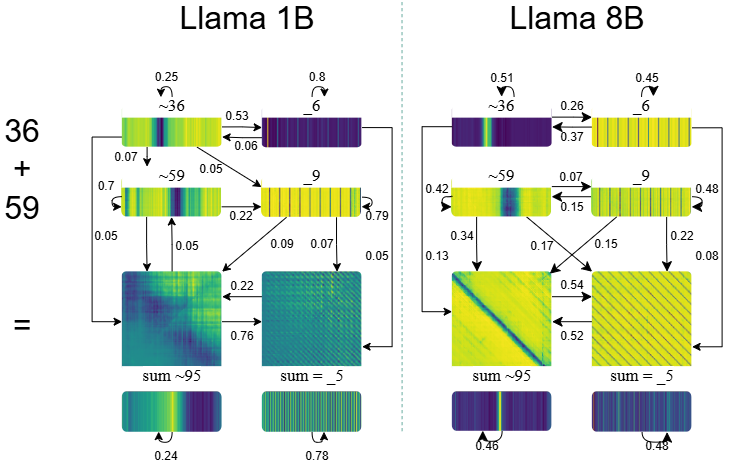
\includegraphics[width=0.84\linewidth]{figures/graph_dist_heatmaps.png}
  \caption{Supergraphs for the prompt ``\texttt{36+59=}'' in Llama-3.2-1B (left) and
  Llama-3.1-8B (right). Each node is a supernode from Section~\ref{sec:supernodes}, drawn as the
  activation grid $T_i$ of one representative member neuron --- its activation across all $10^4$
  two-digit addition prompts, with operand $a$ on one axis and $b$ on the other --- so that
  membership and computational role can be read off the same picture. Nodes $\sim\!36$ and
  $\sim\!59$ are \texttt{arg1/arg2 range}, $\_6$ and $\_9$ are \texttt{arg1/arg2 units},
  $\mathrm{sum}\sim\!95$ and $\mathrm{sum}=\_5$ are \texttt{sum range} and \texttt{sum units}, and
  the bottom pair are the corresponding \texttt{dla} supernodes. Edge labels are the supernode
  weights of \eqref{eq:superedge}; self-loops are within-supernode recurrence. The 8B grids are
  visibly cleaner: its $\mathrm{sum}\sim\!95$ node is a sharp anti-diagonal ($a + b \approx 95$) and
  its $\mathrm{sum}=\_5$ node a clean periodic lattice ($a + b \equiv 5 \bmod 10$), whereas the 1B
  counterparts are diffuse and noisy --- the same structure, represented less separably in the
  smaller model.}
  \label{fig:supergraph}
\end{figure}

\subsection{Supernode edge weights}
\label{sec:superedges}

The supergraph's edges are the supernode adjacency of \citet{ameisen2025circuit},
\begin{equation}
  \snadj(t,s)
  \;=\;
  \frac{\displaystyle\sum_{n_t \in N_t} \fracext(n_t) \cdot \sum_{n_s \in N_s} A'_{n_t, n_s}}
       {\displaystyle\sum_{n_t \in N_t} \fracext(n_t)},
  \label{eq:superedge}
\end{equation}
where $N_t$ and $N_s$ are the member nodes of supernodes $t$ and $s$, and $A'$ is the graph
adjacency with each node's incoming weights normalised to sum to one over \emph{all} sources ---
neurons, token embeddings and logits alike. The weight $\fracext(n_t)$ is the fraction of a
member's absolute inbound weight that comes from outside its own supernode, so members that mainly
feed one another count for little and a supernode cannot dominate its own inbound profile. Because
$A'$ normalises over all nodes while the supergraph spans only supernode columns, the rows of
$\snadj$ do not sum to one, which is why the routing profiles of Section~\ref{sec:overview}
renormalise them.

Implementation details --- adapting the attribution pipeline to Llama's gated MLPs and Hugging Face
autograd, and the optimisations that make it fast enough for a training loop --- are given in
Appendices~\ref{app:llama} and~\ref{app:perf}.

\section{Experimental Setup}
\label{sec:setup}

The teacher is Meta-Llama-3-8B-Instruct and the student Llama-3.2-1B-Instruct, both public
checkpoints; the teacher is frozen and runs in bf16, the student holds fp32 master weights under a
bf16 autocast forward (Appendix~\ref{app:llama}). Training prompts are two-digit additions
``\texttt{$a$+$b$=}'' (22\_add), batch 32, AdamW at $10^{-6}$ with no schedule, 100 steps.
Generalisation is measured on four families never seen in training: three- and four-operand sums
of two-digit numbers (222\_add, 2222\_add), three-digit addition (33\_add) and two-digit by
one-digit multiplication (21\_mult), $5000$ held-out prompts each ($1000$ for 21\_mult), scored by
greedy decoding and exact match on the leading integer of the continuation. We compare three
objectives through one trainer stack: supervised fine-tuning on the gold answers (SFT); standard
KD from the teacher's logits at $\tau = 2$; KD plus the graph loss \eqref{eq:total} with
$\lambda = 0.1$ and the prompt-derived supernodes of Section~\ref{sec:supernodes-general}; and,
as representation-level references that constrain the student's internals without a graph, KD
plus the TinyBERT recipe \citep{jiao2020tinybert} --- mean-squared error between a learned linear
projection of the student's residual stream and the teacher's at uniformly mapped layers, plus
attention-pattern MSE at the same layers --- and KD plus linear centred kernel alignment
\citep{kornblith2019similarity} on the residual streams, both at weight $0.1$ in place of $\lambda$. Every
baseline carries three seeds and the distillation baselines train for 300 steps so that their
later peaks are not cut off. The full configuration is Table~\ref{tab:config}.

\todosec{Still to add: hardware and wall-clock cost per step for each objective.}

\section{Results}
\label{sec:results}

Table~\ref{tab:main} and Figure~\ref{fig:main} compare the objectives. Graph distillation
reaches $0.983$ in-distribution and $0.525$ mean held-out accuracy at step 100, against
$0.976 \pm 0.028$ and $0.415 \pm 0.025$ for SFT and $0.900 \pm 0.011$ and $0.369 \pm 0.022$ for
standard KD. The held-out margin over SFT is $0.11$, about four SFT seed standard deviations, and
holds on three of the four families; on 33\_add SFT is ahead at step 100, with the largest seed
spread of any cell in the table. The margin over standard KD is $0.16$ at matched steps and $0.14$
against the control's later peak at step 160, and graph distillation reaches its own peak at step
85. On 21\_mult, the one held-out family that is not addition, graph distillation nearly matches
the teacher's in-distribution accuracy while every baseline stops near $0.55$.

Constraining the student's internals is not by itself what helps. The two representation-level
baselines, which add a hidden-state loss to the same KD term at the same weight, land at or below
standard KD: $0.309 \pm 0.003$ mean held-out accuracy at step 100 for the TinyBERT recipe and
$0.341 \pm 0.004$ for CKA, with peaks of $0.375$ and $0.373$ against the control's $0.383$, and
in-distribution accuracy within $0.02$ of the control throughout. Both dip exactly as standard KD
does. What the graph term adds is therefore not a generic regulariser on the residual stream but
something specific to the routing target, and Appendix~\ref{app:lambda} tests that directly by
scrambling the target.

\begin{table}[t]
  \centering
  \small
  \caption{Accuracy at step 100 on the training family (22\_add) and the four held-out families,
  the mean over the held-out families, and the peaks over the run with their step. Seed mean
  $\pm$ sd over three seeds for the baselines; the graph run is a single seed. The three
  distillation baselines trained to step 300; the teacher scores $0.957$ on 22\_add. Bold is the
  best mean in a row; italics are below the untrained student.
  \emph{Dip / recovery} is the minimum in-distribution accuracy over steps 1--40 and the first
  later step back at or above the untrained student.}
  \label{tab:main}
  \scriptsize\setlength{\tabcolsep}{1.5pt}
  \tablerows{main_results}
\end{table}

\begin{figure}[t]
  \centering
  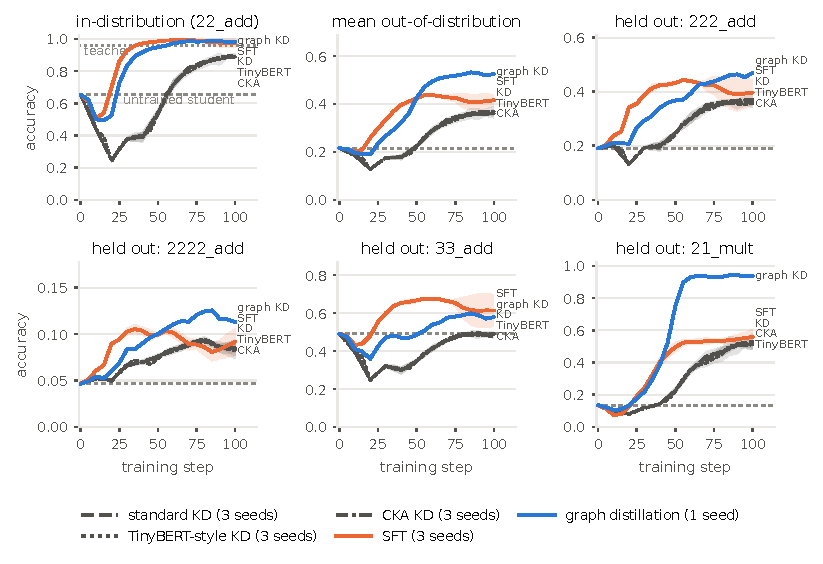
\includegraphics[width=\textwidth]{figures/main_results.pdf}
  \caption{Accuracy against training step: in-distribution, the mean over the four held-out
  families, and each family. The three distillation baselines share the grey of the reference
  method and differ in line style; seed means with a $\pm 1$ sd band for the three-seed
  baselines. The dashed rule is the untrained student and the dotted rule the teacher.
  Every run dips below the untrained student before recovering; the dip is deepest and longest for
  standard KD and the graph term removes most of it (Appendix~\ref{app:lambda}).}
  \label{fig:main}
\end{figure}

Standard KD is the weaker baseline on every measure. It falls to $0.25$ in-distribution in its first
twenty steps and needs sixty to recover the untrained student, where SFT and graph distillation
dip to about $0.50$ and recover by step 25; it never reaches SFT's held-out peak in three times the
steps. The graph term is what closes that gap: Appendix~\ref{app:lambda} shows the dip shrinking
monotonically with $\lambda$ and the held-out gain appearing only once a run has recovered.
Appendix~\ref{app:freeze} shows that the choice of linearisation inside the attribution does not
change the outcome at the working weight.

\pending{: seeds 2--3 for graph distillation, on which the error bars of its row depend.}

\todosec{Still to add: graph-loss and KD-loss curves; whether supernode routing converges toward
the teacher's; per-supernode breakdown of which routes align and which do not.}

\section{Analysis}
\label{sec:analysis}

\todosec{Analysis. Qualitative before/after supergraphs for the student; do the student's
activation grids sharpen over training? Ablations beyond $\lambda$ (Appendix~\ref{app:lambda})
and the linearisation (Appendix~\ref{app:freeze}): JSD vs.\ other divergences, number of
supernodes, $n_{\mathrm{per}}$.}

\section{Limitations}
\label{sec:limitations}

\todosec{Limitations. Single task family (two-digit addition) and a single teacher/student pair;
attribution graphs are built per prompt and only at sampled positions; edge sign is discarded by
the input normalisation; supernode membership is recomputed but not itself differentiable.}

\section{Conclusion}
\label{sec:conclusion}

\todosec{Conclusion.}

% ICLR 2027: the AI use statement is required; the ethics and reproducibility
% statements are recommended. None of the three counts toward the page limit,
% and all go at the end of the main text, before the references.

\subsection*{AI use statement}

\todosec{AI use statement (required by ICLR 2027; see the AI Policy for Authors).
State which of the tasks with required disclosure generative AI was used for and
which it was not, how AI-assisted work was reviewed, and that the authors take
responsibility for the final content.}

\subsection*{Ethics statement}

\todosec{Ethics statement (recommended). Synthetic arithmetic data, public model
checkpoints, no human subjects; note anything the Code of Ethics asks about.}

\subsection*{Reproducibility statement}

\todosec{Reproducibility statement (recommended). Point to the appendices that
carry the full hyperparameters, the training precision regime, the supernode
construction and the diagnostics, and to the anonymised code in the supplementary
material.}

\bibliography{references}
\bibliographystyle{iclr2027_conference}

\appendix

% Every table in the appendices is \input from latex/graph_distillation/tables/,
% which the scripts in src/experiments/plot_*.py regenerate from the training
% histories together with the figures. Re-run them after any new run lands:
%   PYTHONPATH=src python -m experiments.plot_main_results
%   PYTHONPATH=src python -m experiments.plot_lambda_sweep
%   PYTHONPATH=src python -m experiments.plot_freeze_ablation
%   PYTHONPATH=src python -m experiments.plot_grad_metrics
%   PYTHONPATH=src python -m experiments.plot_scramble
% Slots waiting on a run are marked \pending{} and listed in Appendix F.

\section{Adapting the Pipeline to Llama}
\label{app:llama}

The published methodology assumes a transcoder replacement model and a TransformerLens-style hook
API \citep{ameisen2025circuit}. Running it inside a Hugging Face training loop on Llama required
several changes, most forced by the requirement that the student's graph carry gradients back into
$\theta_\Stud$.

\emph{Gated MLPs.} Llama's MLP is a SwiGLU block \citep{shazeer2020glu} with no single input matrix.
With residual-stream input $h$ at the node's position,
\begin{equation}
  a_i = \sigma(g_i)\, u_i, \qquad
  v^{\mathrm{in}}_i = \frac{\partial a_i}{\partial h}
    = \sigma(g_i)\, W_{\mathrm{up}}[n_i,:] \;+\; u_i\,\sigma'(g_i)\, W_{\mathrm{gate}}[n_i,:],
  \label{eq:swiglu}
\end{equation}
where $g_i = \langle W_{\mathrm{gate}}[n_i,:], h\rangle$, $u_i = \langle W_{\mathrm{up}}[n_i,:],
h\rangle$ and $\sigma$ is SiLU. The read direction is therefore a product-rule sum of two terms that
itself depends on the activation, rather than a fixed row of $W_{\mathrm{in}}$.

\emph{Differentiability.} The pre-selection top-$k$ is detached (indices are not differentiable),
but activations and read/write vectors stay in the ambient autograd context, so gradients flow
$\mathcal{L}_{\mathrm{graph}} \to \snadj \to A' \to A \to v^{\mathrm{out}} \to W_{\mathrm{down}}$
back into the model. Supernode \emph{membership} is recomputed each step but treated as fixed
structure; only the aggregation \eqref{eq:superedge} is rebuilt differentiably, out-of-place, so
that autograd views survive.

\emph{Shared attribution targets.} Both models are attributed to the \emph{same} logit token set ---
the teacher's --- and the student's \texttt{dla} supernodes are selected against the teacher's
logits. Otherwise the two graphs would be built over different output nodes, and would be
non-stationary early in training when the student's own output distribution is still wrong.

\emph{Linearisation.} The published method freezes attention patterns and normalisation
denominators when linearising, so that edges reflect only the direct residual-stream path. We
implement both freezes as backward-only stop-gradients and make each independently selectable, so
\eqref{eq:edge} can be evaluated either with the direct-path linearisation or through the full
Hugging Face Jacobian. Appendix~\ref{app:freeze} measures what the choice costs at the working
$\lambda$: at initialisation it rotates the graph gradient by $40^\circ$ to $50^\circ$, and over a
full run it changes downstream accuracy by less than the seed-to-seed spread of the baselines.

\emph{Precision.} The graph gradient is small next to the KD gradient --- under $1\%$ of its norm
at step one and a few per cent by the end of a run for $\lambda \in [0.03, 0.3]$
(Table~\ref{tab:freeze-dynamics}) --- and it arrives one prompt at a time, since each prompt's
graph is backpropagated and freed before the next is built (Appendix~\ref{app:perf}). With bf16
parameters those $\sim$32 partial sums each land below half a unit in the last place of a
\texttt{.grad} buffer that already holds the KD gradient, and are rounded away: we measured only
$66$--$100\%$ of the graph gradient surviving accumulation, decreasing with $\lambda$, which
silently compressed a $\lambda$ sweep toward its top. bf16 weights lose the update itself as well,
since an AdamW step at $10^{-6}$ is under half a ULP for most weights; only about $2\%$ of the
parameters changed on a step. The student therefore holds fp32 master weights and fp32 optimiser
moments and runs its forward under bf16 autocast; the inference-only teacher stays bf16. Every run
records the fraction of parameters that moved on step one as a canary (it is $1.000$ for every run
reported here), and the step-one check of Appendix~\ref{app:lambda} confirms that scale-invariant
summaries of the graph gradient agree across $\lambda$.


\section{The Direct-Path Linearisation as a Training Signal}
\label{app:freeze}

Circuit tracing freezes attention patterns and RMSNorm denominators so that an edge is the
contribution of the direct path alone \citep{ameisen2025circuit}. That choice is made for
interpretability: it renders the graph locally linear in the node activations and therefore
readable. It is not obvious that it is also the right choice when the graph is a regression target
rather than a figure, since the frozen edge omits real causal influence --- paths on which a source
node shifts \emph{where} a target attends, and the rank-one RMSNorm term that projects out the
component of each edge along the activation direction. This appendix measures the difference,
first in the gradient the choice produces and then in the student it trains.

\subsection{Implementation}

Both freezes are backward-only. Detaching a multiplicative factor leaves every forward value
bit-identical, so activations, read and write vectors, neuron pre-selection and supernode membership
are unchanged; only the gradients that become edge weights differ. Freezing attention additionally
requires a kernel that materialises the pattern, since the default fused kernel never forms it.

One implementation detail is load-bearing. Attribution involves two forward passes: one whose
captured MLP inputs carry gradient back to $\theta_\Stud$, and one whose \emph{backward} produces
the edge values of \eqref{eq:edge}. The freeze belongs only on the second. Applied to the first it
cannot change any edge --- being backward-only, it changes no forward value --- but it silently
biases training, zeroing the gradient to $W_Q$ and $W_K$ outright and stripping the rank-one
correction from every RMSNorm on the path back to the weights. We hit this: with the freeze on both
passes, in-distribution accuracy collapsed from $0.634$ to $0.090$ within twenty steps while the KD
loss continued to fall.

The RMSNorm freeze has a second, measurable effect on the \emph{target}. Frozen minus true
Jacobian is $+r\,\hat{x}\hat{x}^{\top}$, a rank-one radial term, and in Llama $\hat{x}$ is dominated
by the massive activations at the attention sink. Frozen edges therefore load onto the BOS node
(its share of attribution mass rises from $0.11$ to $0.47$ in the teacher and from $0.07$ to
$0.53$ in the student), which saturates every member's $\fracext$ near $1$ and collapses the
member weighting of \eqref{eq:superedge} to a plain mean. The ablation below therefore includes an
arm that keeps the unfrozen Jacobian but sets the weighting to a constant, to separate the freeze's
effect on the target from its effect on the gradient.

\subsection{Gradient geometry at initialisation}

Table~\ref{tab:freeze-grad} reports the graph gradient under each variant at the student's initial
checkpoint, against the unfrozen gradient and against the KD gradient.

\begin{table}[h]
  \centering
  \caption{Graph-loss gradient under each linearisation, at the student's initial checkpoint;
  22\_add, 8 graph prompts, $\lambda_{\mathrm{graph}}=1$. Cosines are against the unfrozen graph
  gradient and against the KD gradient. Measured with the earlier bf16 gradient accumulation
  (Appendix~\ref{app:llama}), which attenuates the graph gradient's magnitude but not its
  direction. \pending{: re-measure in the fp32 regime.}}
  \label{tab:freeze-grad}
  \begin{tabular}{lccccc}
    \toprule
    & $\mathcal{L}$ & $\|g\|$ & $\|g\|/\|g_{\mathrm{unfr}}\|$ & $\cos(g, g_{\mathrm{unfr}})$ & $\cos(g, g_{\mathrm{KD}})$ \\
    \midrule
    $\mathcal{L}_{\mathrm{KD}}$ & 2.0254 & 50.41 & --- & --- & --- \\
    \midrule
    unfrozen                    & 0.3405 & 3.647 & 1.000 & $+1.0000$ & $-0.0236$ \\
    attention frozen            & 0.3501 & 4.059 & 1.113 & $+0.6276$ & $-0.0103$ \\
    RMSNorm frozen              & 0.3722 & 3.991 & 1.094 & $+0.7652$ & $-0.0153$ \\
    both frozen                 & 0.3745 & 3.856 & 1.057 & $+0.6984$ & $-0.0082$ \\
    \bottomrule
  \end{tabular}
\end{table}

The freeze changes direction, not strength: every frozen variant is $40^\circ$ to $51^\circ$ away
from the unfrozen gradient while being slightly \emph{larger} in norm. The unfrozen total-effect
gradient is the smallest of the four, which is what destructive interference between paths
produces --- freezing removes the cancellation rather than removing signal. The two freezes also
partially cancel each other: freezing both gives a smaller gradient than either alone and an angle
between the two. A plausible mechanism is that the RMSNorm freeze injects the radial sensitivity
described above, while the attention freeze deletes the QK path, the channel most responsive to a
radial perturbation because rescaling the query sharpens or flattens the softmax. Whether a
$45^\circ$ rotation of a gradient this small matters to training is the question the next section
answers.

\subsection{Training ablation}
\label{sec:freeze-train}

Table~\ref{tab:freeze-train} and Figure~\ref{fig:freeze-ablation} train the variants for 100
steps at the working weight $\lambda = 0.1$ under otherwise identical settings (those of
Appendix~\ref{app:lambda}), evaluating in-distribution on two-digit addition and out-of-distribution
on four arithmetic families never seen in training.

\begin{table}[h]
  \centering
  \small
  \caption{Distillation accuracy under each linearisation at $\lambda = 0.1$, step 100, laid out
  as Table~\ref{tab:main}. Single seed per arm; the two arms not yet run are marked.}
  \label{tab:freeze-train}
  \footnotesize\setlength{\tabcolsep}{4pt}
  \tablerows{freeze_train}
\end{table}

\begin{figure}[h]
  \centering
  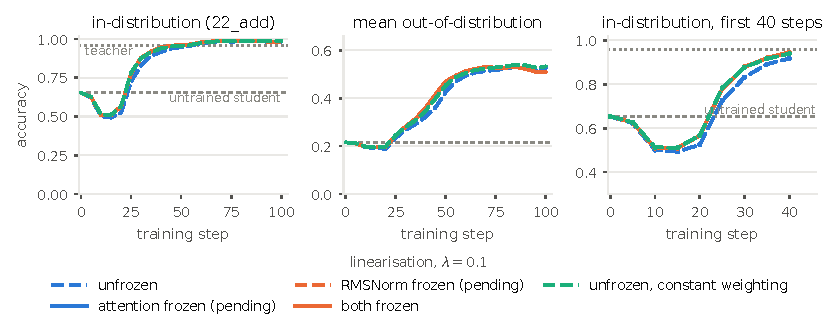
\includegraphics[width=\textwidth]{figures/freeze_ablation.pdf}
  \caption{Accuracy against training step for the linearisation arms at $\lambda = 0.1$. Hue
  carries the RMSNorm freeze and line style the attention freeze, so the 2$\times$2 design reads as
  two pairs; the constant-weighting arm is the third hue. \emph{Left, centre}: the full run;
  \emph{right}: the first forty steps of the in-distribution curve, where the arms differ most.
  The dashed rule is the untrained student and the dotted rule the teacher. The arms lie on top
  of one another: that overlap is the result.}
  \label{fig:freeze-ablation}
\end{figure}

At the working weight the linearisation does not change what the student learns. The three arms
run so far end within $0.022$ mean OOD of one another at step 100 and within $0.008$ at their
peaks, which all fall at step 85; their in-distribution accuracies are within $0.003$. That spread is
smaller than the seed-to-seed standard deviation of the baselines in Section~\ref{sec:results}
($0.025$ mean OOD for SFT over three seeds), so no ordering among them can be claimed from one
seed. Two things do separate the arms. Both the freeze and the constant weighting shallow the dip
that every run takes before recovering (Appendix~\ref{app:lambda}): the minimum rises from
$0.493$ to $0.509$ and $0.511$, and the both-frozen arm reaches it five steps sooner. And the
both-frozen arm is the only one to lose ground after its peak, giving back about $0.03$ on each of
222\_add and 2222\_add between steps 70 and 100 where the other two are flat or still rising.

The constant-weighting arm is the informative null. It reproduces the unfrozen arm to within
$0.008$ on every family, so the $\fracext$ weighting of \eqref{eq:superedge} is inert here, and by
the same token the RMSNorm freeze's saturation of that weighting cannot be what any RMSNorm-frozen
arm is doing. Whatever the freeze contributes must come through the gradient, and at this
$\lambda$ that contribution is inside noise.

This reverses an earlier reading. An ablation at $\lambda = 1$, 15 steps, under the bf16
accumulation of Appendix~\ref{app:llama}, had ranked the arms monotonically with the amount frozen.
That measurement ordered the arms by the depth of the dip --- at 15 steps there is no OOD signal
yet, since no run has recovered the untrained student --- and, as Table~\ref{tab:freeze-train}
shows, the freeze does shallow the dip. It is the extrapolation from the dip to generalisation
that did not hold.

\pending{: the attention-only and RMSNorm-only arms at $\lambda = 0.1$; seeds 2--3 for the
unfrozen and both-frozen arms; one both-frozen run at $\lambda = 0.3$, where the graph gradient is
three times larger and a rotation of it would have more room to matter.}

\subsection{Gradient dynamics over training}
\label{sec:freeze-dynamics}

Every run records per-step gradient instrumentation. Figure~\ref{fig:grad-metrics} plots it and
Table~\ref{tab:freeze-dynamics} summarises it.

\begin{table}[h]
  \centering
  \caption{Per-step gradient metrics averaged over the 100 steps, $\lambda = 0.1$. The graph norm
  is already scaled by $\lambda$, so these are the quantities that reach the optimiser; the
  cosine column gives the signed mean and, in parentheses, the mean absolute value.}
  \label{tab:freeze-dynamics}
  \small
  \begin{tabular}{lccccc}
    \toprule
    & $\|g_{\mathrm{KD}}\|$ & $\lambda\|g_{\mathrm{graph}}\|$ & ratio & $\cos$ (mean $|\cos|$) & sign flips \\
    \midrule
    \tablerows{freeze_dynamics}
    \bottomrule
  \end{tabular}
\end{table}

\begin{figure}[h]
  \centering
  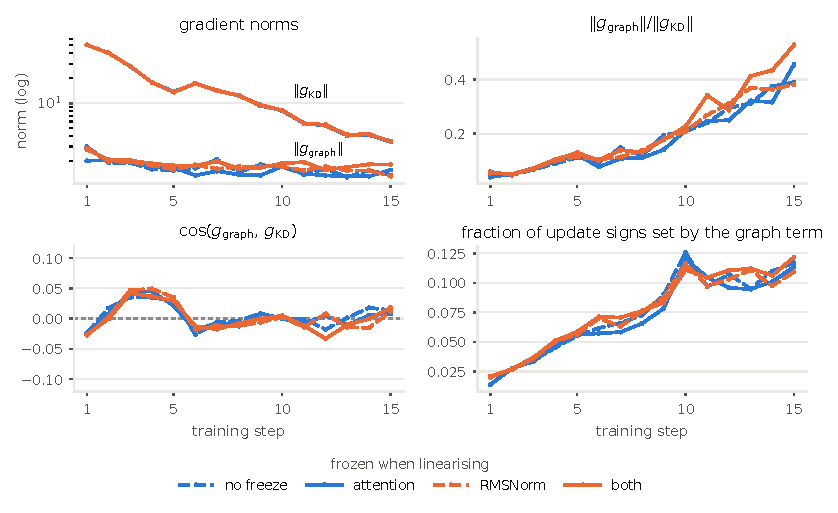
\includegraphics[width=\textwidth]{figures/grad_metrics.pdf}
  \caption{Per-step gradient metrics for the linearisation arms, encoded as in
  Figure~\ref{fig:freeze-ablation}. The arms are drawn on every panel and lie on top of one
  another. The KD gradient falls twentyfold while the graph gradient stays within a factor of two,
  so their ratio climbs an order of magnitude and the share of update signs the graph term
  decides rises from $0.3\%$ to $2\%$, none of it by design. The cosine oscillates about zero
  throughout; its excursions coincide across arms because the arms see the same batches.}
  \label{fig:grad-metrics}
\end{figure}

\emph{The graph term progressively takes over.} $\|\nabla\mathcal{L}_{\mathrm{KD}}\|$ falls from
$49.2$ at step one to $2.5$ at step 100, while $\lambda\|\nabla\mathcal{L}_{\mathrm{graph}}\|$
goes from $0.30$ to $0.17$. Their ratio therefore climbs from $0.006$ to $0.07$, with transient
spikes to $0.27$ on individual batches, and the fraction of parameter entries whose update sign
the graph term decides rises from $0.3\%$ to $2.3\%$. Nobody chose this schedule: it is a
consequence of KD converging faster than the graph objective. It also lines up with the accuracy
curves of Appendix~\ref{app:lambda}: in-distribution accuracy is saturated by step 70 in every
graph run while mean OOD accuracy goes on rising to step 85.

\emph{No aggregate gradient statistic separates the arms}, which is consistent with their
identical accuracy: the run means differ by $0.3\%$ in KD norm, $2\%$ in graph norm and about
$5\%$ in ratio and sign flips, and the cosine traces coincide step for step. If the arms differ
at all it is in \emph{which} parameters the graph term moves, and scalar summaries are blind to
that by construction.

One incidental observation: the pre-clip gradient norm never falls below $1.9$ and so exceeds the
clip threshold of $1.0$ at every step of every run. Gradient clipping is not a rarely-triggered
safety valve here but a permanent rescaling --- one that AdamW largely undoes, since per-parameter
normalisation cancels a uniform scale factor.

\subsection{Caveats}

Single seed per arm; one supernode construction, the arg-token and DLA supernodes of
Section~\ref{sec:supernodes-general}, not the ANOVA supernodes. The freeze acts on the edge
coefficients, before supernodes are formed, so the RMSNorm result should transfer; the attention
result is less safe to extrapolate, since arg-token supernodes are positional and attention is
the only mechanism that moves information between positions. The gradient geometry of
Table~\ref{tab:freeze-grad} was measured in the earlier bf16 regime. 2222\_add is close to
unlearned in every configuration.


\section{Sensitivity to the Graph-Loss Weight}
\label{app:lambda}

The weight $\lambda$ in \eqref{eq:total} is the one hyperparameter the method adds. We sweep
$\lambda \in \{0.03, 0.1, 0.3\}$ against two references trained through the same stack and
evaluated identically: the $\lambda = 0$ control, which is standard knowledge distillation, and
supervised fine-tuning on the same prompts. Everything else is held fixed: learning rate
$10^{-6}$, batch size 32, $\tau = 2$, the same data order, and the unfrozen arg-token and DLA
supernodes of Section~\ref{sec:supernodes-general} with three neurons each
(Appendix~\ref{app:details} has the full table). The graph runs train for 100 steps; the control
trains for 300 so that its peak is not cut off. Table~\ref{tab:lambda} and Figure~\ref{fig:lambda}
report the result; the references carry three seeds each, the sweep one.

\begin{table}[h]
  \centering
  \small
  \caption{Accuracy under each graph-loss weight against the two references, laid out as
  Table~\ref{tab:main}: families at step 100, peaks over the run with their step, and the
  in-distribution dip and recovery. Seed mean $\pm$ sd for the three-seed references; the sweep
  is one seed each. The control ran to step 300.}
  \label{tab:lambda}
  \scriptsize\setlength{\tabcolsep}{3pt}
  \tablerows{lambda}
\end{table}

\begin{figure}[h]
  \centering
  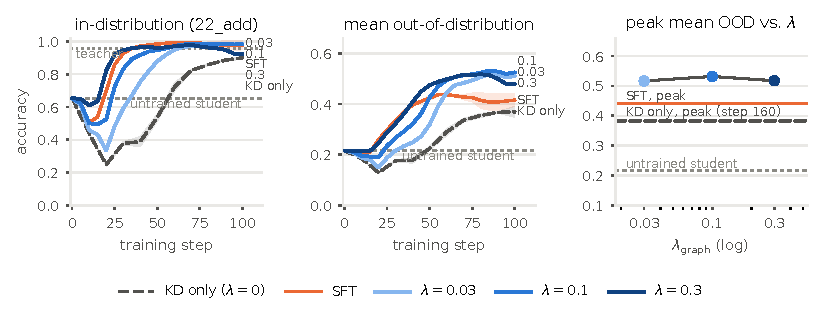
\includegraphics[width=\textwidth]{figures/lambda_sweep.pdf}
  \caption{Sensitivity to $\lambda$. One hue stepped light to dark with increasing $\lambda$;
  standard KD in dashed grey and SFT in orange, seed means with a $\pm 1$ sd band, shown to step
  100 to share the axis. \emph{Left, centre:} in-distribution and mean out-of-distribution accuracy
  against training step; the dashed rule is the untrained student and the dotted rule the teacher.
  \emph{Right:} peak mean out-of-distribution accuracy against $\lambda$ on a log axis, with the
  control's 300-step peak and SFT's peak as reference rules.}
  \label{fig:lambda}
\end{figure}

Three things hold across every metric and every family. First, every graph run beats both
references on every held-out family at step 100, and the margin is not a matter of training
length: the control peaks at $0.383$ mean OOD at step 160 and declines from there, and SFT at
$0.440$ at step 60, against $0.532$ for $\lambda = 0.1$. Standard distillation is in fact the
weaker of the two references here, no better than the untrained student on 33\_add at step 100 and
never reaching SFT's peak in 300 steps. Second, every run first falls below the untrained student
and then recovers, and the dip is monotone in $\lambda$ --- a minimum of $0.248$, $0.335$,
$0.493$ and $0.609$ at $\lambda = 0$, $0.03$, $0.1$ and $0.3$, recovered after 60, 35, 25 and 20
steps --- so the dip belongs to the KD objective and the graph term shortens it. SFT, which has
no KD term, dips only to $0.505$ and recovers by step 20; $\lambda = 0.1$ comes within $0.012$ of
it. Third,
larger $\lambda$ rises faster but peaks earlier and then declines: $\lambda = 0.3$ peaks at step
70--80 and gives back $0.06$ in-distribution and $0.04$ OOD by step 100, while $\lambda = 0.03$
and $0.1$ are flat from step 85. The response is therefore an inverted U whose top is broad ---
the three peaks lie within $0.016$ of one another across a tenfold change in $\lambda$ --- and
what separates the values is stability after the peak rather than the height of it. We use
$\lambda = 0.1$ throughout as the largest weight that has not begun to collapse by step 100.

The sweep doubles as a precision check on the training stack. At step one the runs share weights
and batch, so any scale-invariant summary of the graph gradient must agree across $\lambda$; both
$\|g_{\mathrm{graph}}\| / \lambda$ and $\cos(g_{\mathrm{graph}}, g_{\mathrm{KD}})$ do, to three
decimals ($2.96$ and $-0.015$). Under the bf16 gradient accumulation of an earlier version of the
stack (Appendix~\ref{app:llama}) they did not: the graph gradient, which arrives one prompt at a
time into a buffer already holding the far larger KD gradient, was rounded away more severely the
smaller $\lambda$ was, which biased that regime against small $\lambda$.

\subsection{Structure control: a scrambled target}
\label{sec:scramble}

Does the gain come from the \emph{content} of the teacher's routing, or would any structured
target of the same shape act as a regulariser? We train the $\lambda = 0.1$ configuration against
a scrambled target: each row of the teacher's $K \times K$ supernode adjacency is permuted by a
fixed derangement, drawn once from the run seed and reused for every prompt, so the target keeps
the teacher's numbers and per-row sparsity but pairs every supernode with the wrong sources. The
run also scores the student against the real target at every step, without gradient.
Figure~\ref{fig:scramble} shows the result.

\begin{figure}[h]
  \centering
  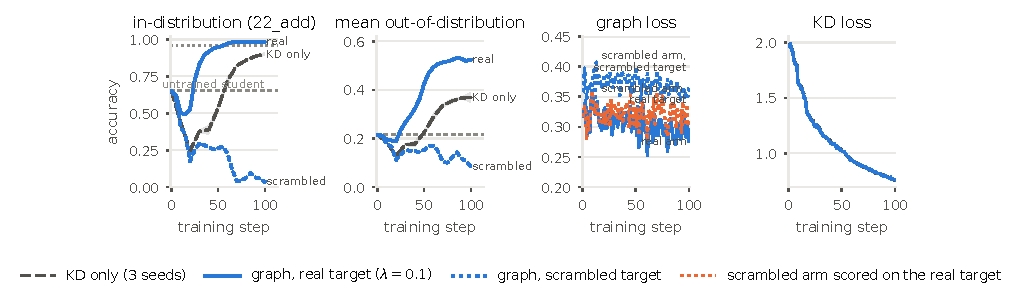
\includegraphics[width=\textwidth]{figures/scramble.pdf}
  \caption{Real against scrambled routing target at $\lambda = 0.1$, single seed, with the KD-only
  control for reference. \emph{Left pair:} accuracy. \emph{Third:} the graph loss the scrambled
  arm trains on, the same arm scored against the real target, and the real arm's loss.
  \emph{Right:} the KD loss of the three runs.}
  \label{fig:scramble}
\end{figure}

The scrambled target is not merely useless but destructive: in-distribution accuracy falls to
$0.036$ by step 100 and mean held-out accuracy to $0.084$, below the untrained student on every
family, while the real target reaches $0.983$ and $0.525$ from the same initialisation, data order
and $\lambda$. This is not a matter of gradient scale --- the scrambled arm's graph gradient is
\emph{smaller} than the real arm's at every stage (step-one ratio to the KD gradient $0.0044$
against $0.0060$, run mean $0.046$ against $0.042$) --- and the student never fits the scrambled
target: its loss on it drifts from $0.358$ to $0.368$ while its loss on the real target stays flat
at $0.31$--$0.33$, where the real arm's falls to $0.276$. A routing target the student cannot
reach still moves the student, and moves it somewhere the teacher's target does not. Together with
the representation-level baselines of Section~\ref{sec:results}, which constrain the same
residual stream to no effect, this locates the gain in the target's content.

\pending{: seeds 2--3 for $\lambda = 0.1$ and for the scrambled arm; $\lambda = 1$ in the fp32
regime.}


\section{Performance Optimisations}
\label{app:perf}

An attribution graph costs one batch-expanded forward pass plus a vector--Jacobian product per node,
which makes $\mathcal{L}_{\mathrm{graph}}$ far more expensive per prompt than $\mathcal{L}_{\mathrm{KD}}$.
Four optimisations bring it inside a training loop. \emph{Probe-set caching:} the residual-stream
input to every MLP over all $10^4$ prompts is computed once per model and cached to disk, keyed by
model and dataset, then read back layer-by-layer, so every activation grid is recovered from the
cache rather than by re-running the model. \emph{Analytic pre-selection:} write-vector norms factor
as $\|v^{\mathrm{out}}_i\|_2 = |a_i|\,\|W_{\mathrm{down}}[:,n_i]\|_2$, so the top-$k$ runs in
$O(n_{\mathrm{pos}} d_{\mathrm{mlp}})$ space without materialising the
$[n_{\mathrm{pos}}, d_{\mathrm{mlp}}, d]$ tensor of write vectors. \emph{Batching:} one
batch-expanded forward pass serves a whole batch of target nodes, and all masks and activation grids
are scored against each other in a single matmul for \eqref{eq:anova}. \emph{Bounded memory:} only
$n_{\mathrm{graph}}$ prompts per batch get a graph, and each prompt's graph loss is backpropagated
and freed before the next graph is built, so peak memory is set by one prompt's attribution graph
rather than the batch's.

\pending{: wall-clock and FLOPs per step for each objective, from \texttt{-{}-track-flops}.}


\section{Training and Evaluation Details}
\label{app:details}

\begin{table}[h]
  \centering
  \small
  \caption{Configuration shared by every run in the paper unless a section says otherwise. The
  three trainers (SFT, standard KD, graph distillation) share one implementation of the
  optimiser, precision regime, data order and evaluation.}
  \label{tab:config}
  \begin{tabular}{ll}
    \toprule
    teacher / student & Meta-Llama-3-8B-Instruct / Llama-3.2-1B-Instruct, $1.24$B parameters \\
    training data & 22\_add prompts ``\texttt{$a$+$b$=}'', batch 32, 100 steps (control: 300) \\
    optimiser & AdamW, learning rate $10^{-6}$, no schedule, gradient clipping at $1.0$ \\
    precision & fp32 master weights and optimiser moments, bf16 autocast forward; teacher bf16 \\
    KD term & $\tau = 2$, forward KL over all non-padding positions \\
    graph term & $\lambda = 0.1$, JSD, arg-token + DLA supernodes, 3 neurons per label \\
    attribution & top $10\%$ of neurons per layer by write norm in the teacher, $1\%$ in the student; \\
                & logit targets: top tokens covering $0.95$ of $\softmax(z/\tau)$, at most ten \\
    linearisation & unfrozen (full Jacobian) unless stated; Appendix~\ref{app:freeze} \\
    evaluation & greedy decoding, up to 5 new tokens, first integer of the continuation; \\
               & every 5 steps (control: 10) on 22\_add and the four held-out families \\
    test sets & $5000$ prompts per family ($1000$ for 21\_mult), disjoint from training \\
    baselines & TinyBERT recipe (MSE on projected hidden states and on attention patterns, \\
              & uniform layer map) and linear CKA on residual streams; weight $0.1$ on the KD term \\
    seeds & 1 for graph runs; 1, 2, 3 for SFT, the KD control and the two representation baselines \\
    \bottomrule
  \end{tabular}
\end{table}

\emph{Evaluation.} An answer is scored by decoding only the generated continuation and parsing its
leading integer. This matters more than it sounds: Llama~3 tokenises digits in groups of one to
three, and the untrained student often emits an answer digit by digit, so a one-token budget
truncates it, while parsing the prompt echo lets a second, echoed equation override a correct
answer. Both effects moved every family's accuracy, the untrained student's included, so all
numbers in the paper come from one evaluation convention and are not comparable to earlier drafts.

\emph{Held-out families.} 222\_add and 2222\_add are three- and four-operand sums of two-digit
numbers, 33\_add is three-digit addition (the only family whose answers need two tokens), and
21\_mult is a two-digit by one-digit product.

\emph{Pending results.} The following slots are marked \pending{} in the text and will be filled
from the same scripts without editing the tables by hand: seeds 2--3 for the $\lambda = 0.1$ run
and for the scrambled arm (Section~\ref{sec:results}, Appendix~\ref{app:lambda}); the
attention-only and RMSNorm-only linearisation arms and seeds for the both-frozen arm
(Appendix~\ref{app:freeze}); the fp32 re-measurement of Table~\ref{tab:freeze-grad}; FLOPs per
step (Appendix~\ref{app:perf}).

\todosec{Still to write: the complete ANOVA category list including the composite and
combination-sum categories omitted from Section~\ref{sec:supernodes}; additional supergraph
figures; per-supernode activation-heatmap montages.}

\end{document}
